\chapter{Ectopic activation of the spindle assembly checkpoint reveals its dose-response characteristics}
\label{chpt2}

Ideally, the SAC should respond to a single unattached (or laterally attached) kinetochore in a dividing cell. Indeed, a single unattached kinetochore delays anaphase onset in mitotic PtK1 cells \cite{PtK1SingleUnattachedKT}. However, the SAC may be less stringent in the first few cleavages of mammalian zygotes \cite{MouseEmbryoSAC, ParentalGenomeUnification}. To understand how the SAC responds to the changing number of signaling kinetochores over the progression of mitosis (\myref{SACRole}), it is necessary to quantify its dose-response characteristics. However, it is technically demanding to maintain a specific number of signaling kinetochores in the cells \cite{Ablation}, especially when a large number of cells are required to counter the noise.

This chapter describes a novel ectopic SAC (eSAC) activator, which activates the SAC independently of the status of kinetochore-microtubule attachment in human cells. By exploiting heterogeneous expression of eSAC activators in a large population of cells, we defined the dependence of the eSAC activator-induced mitotic arrest on the abundance of the eSAC activator to reveal the dose-response characteristics of the core SAC signaling cascade. The critical role of cooperativity is implied in modulating how the SAC responds to the changing number of signaling kinetochores to achieve aforementioned sensitivity in the mitosis of somatic cells.

This chapter is paraphrased and adapted from \cite{eSAC}, with the addition of new references and some of my unpublished data. Key experiments and data mentioned in this chapter to which I am not a main contributor are referred back to the published paper and credited accordingly (those figures are not reproduced here). Certain statements in the original discussion have been adjusted to reflect the up-to-date understanding of the SAC. However, the basic ideas and main conclusions stay the same as in the original paper.

\section{Engineering an ectopic SAC (eSAC) activator}
The SAC signaling is initiated by the phosphorylation of MELT motifs in \protein{Knl1} by \protein{Mps1} at unattached (or laterally-attached) kinetochores \cite{MPS1-KNL1_London2012, MPS1-KNL1_Shepperd2012, MPS1-KNL1_Yamagishi2012, GSK923295MonastrolCotreatment, GSK923295LateralAttachmentEM, LateralAttachmentSAC}. It should be possible to bypass the involvement of kinetochores and activate the SAC signaling by bringing \protein{Mps1} into close proximity with \protein{Knl1}. Previous studies have shown that the SAC can be activated ectopically (independently of the status of kinetochore-microtubule attachment) by overexpressing Mps1 in the budding yeast \cite{Mps1pOverexpressionActivatesSAC}, anchoring \protein{Mad1} to metaphase kinetochores in human cells \cite{HeLa-A12_Ballister2014}, or dimerizing Knl1 with Mps1 in the budding yeast \cite{BuddingYeasteSAC} or the fission yeast \cite{FissionYeasteSAC}. Inspired by these results, we engineered an ectopic SAC (eSAC) activator consisting of a recombinant \protein{Knl1} phosphodomain and a recombinant \protein{Mps1} kinase domain (\myref{eSAC}). They are fused with the chemical-induced dimerization system, wherein FKBP and FRB bind to each other in a rapamycin-dependent manner with high specificity and affinity \cite{FKBP-Rapamycin-FRB}.

\begin{figure}
    \centering
    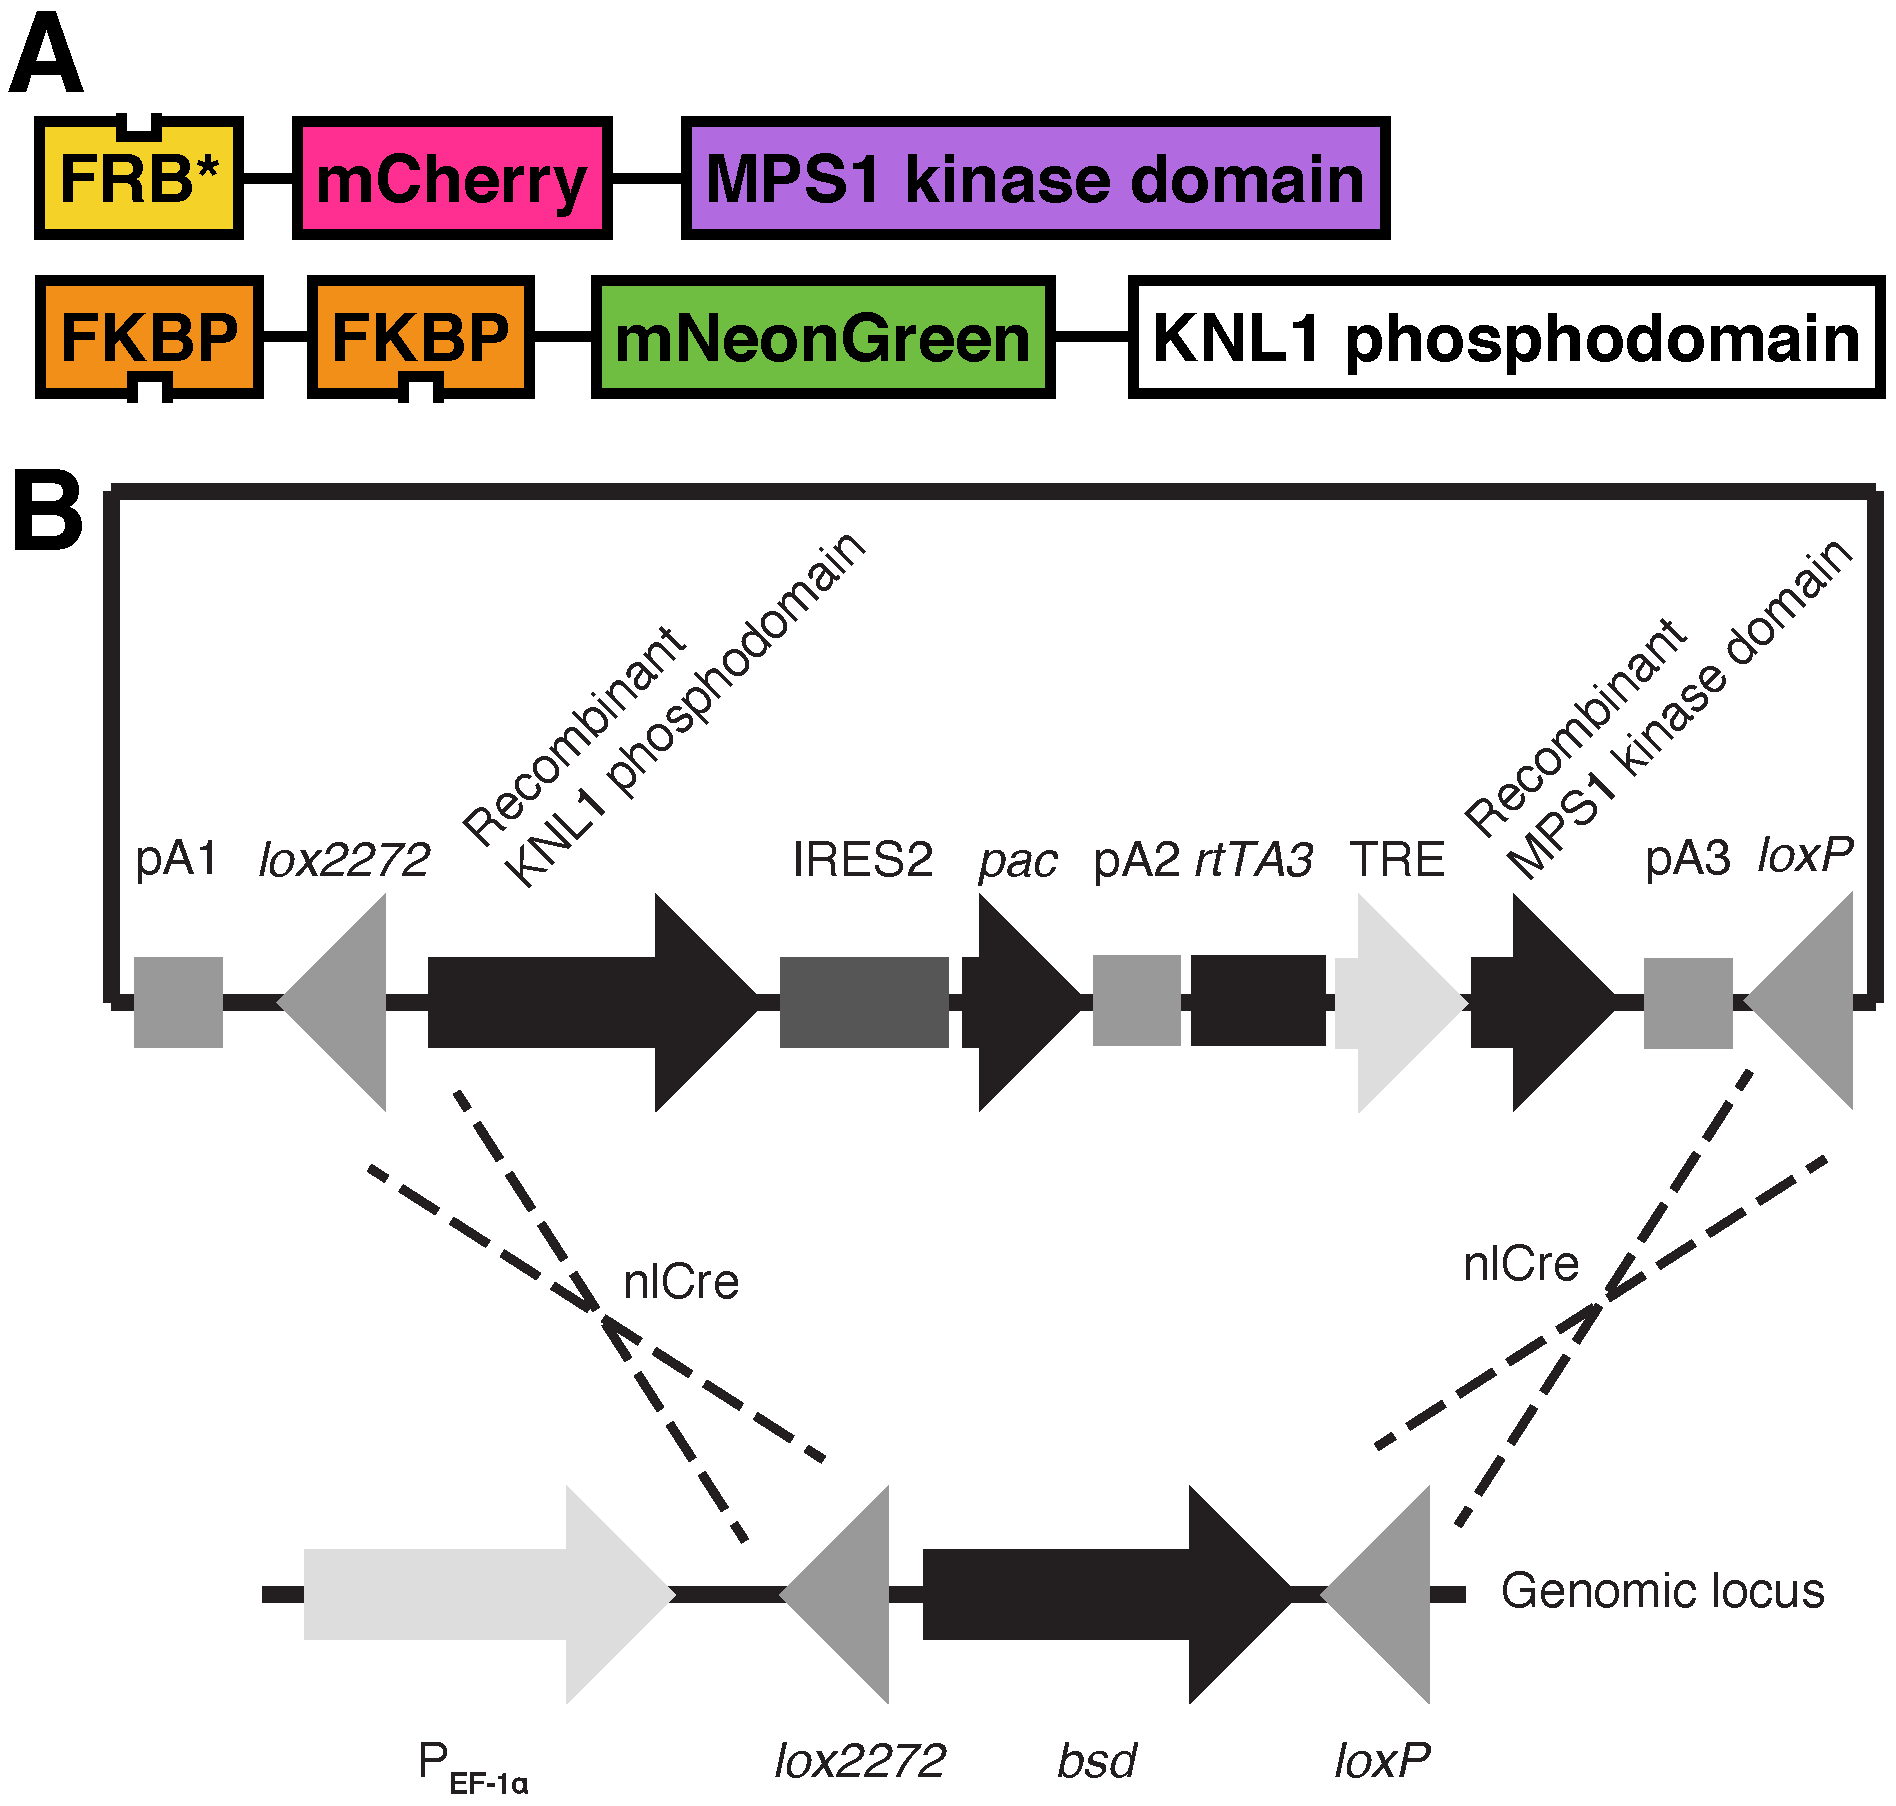
\includegraphics[width=0.7\textwidth]{chapters/figures/eSAC+Cre-lox.pdf}
    \phantomsubfiglabel{eSAC} % subfigure A
    \phantomsubfiglabel{Cre-lox} % subfigure B
    \caption{\textbf{The design of an ectopic SAC (eSAC) activator.}}
    \noindent\justifying (A) The eSAC activator consists of a recombinant \protein{Knl1} phosphodomain and a recombinant \protein{Mps1} kinase domain. The phosphodomain is at the N-terminus of the corresponding recombinant protein while the kinase domain is at the C-terminus of the corresponding recombinant protein. (B) A diagram demonstrating Cre-\bacterialgene{lox} recombination-mediated cassette exchange (RMCE) between a transfected circular plasmid (the top part) and the genomic locus (the bottom part). This diagram is not to scale. The design was adapted from \cite{HeLa-A12_Khandelia2011, HeLa-A12_Ballister2014}. pA1: the polyadenylation signal of herpes simplex virus thymidine kinase. IRES2: (encephalomyocarditis virus) internal ribosome entry site 2. \bacterialgene{pac}: the coding sequence of puromycin \textit{N}-acetyltransferase. pA2: the polyadenylation signal of bovine growth hormone. \textit{rtTA3}: an expression cassette encoding the reverse tetracycline-controlled transactivator 3 (rtTA3), consisting of the promoter of the human ubiquitin C gene, the coding sequence of rtTA3, and a polyadenylation signal from simian virus 40. TRE: a tetracycline-responsive promoter element consisting of six tandem tetracycline operators followed by the minimal promoter sequence derived from the human cytomegalovirus immediate-early promoter. pA3: the polyadenylation signal of rabbit \textbeta{}-globin. nlCre: nucleus-localized Cre recombinase. P\textsubscript{EF-1\textalpha{}}: promoter of the human \gene{EF1A} gene. \bacterialgene{bsd}: the coding sequence of blasticidin S deaminase. After integrated into the genomic locus, the recombinant phosphodomain is under the regulation of the \gene{EF1A} promoter while the recombinant kinase domain is under the regulation of the TRE. Colonies of stably-transfected cells selected by \SI{0.5}{\micro g/mL} -- \SI{2}{\micro g/mL} of puromycin in a well were pooled together to make an eSAC cell line.
    \label{eSAC+Cre-lox}
\end{figure}

The kinetochore targeting of \protein{Knl1} is mainly mediated by its C-terminus \cite{KNL1CTer_Kiyomitsu2007, Screpanti2011, Knl1CTer, MIS12CStructure_Petrovic2016, Spc105pCTer-MIND_Maskell2010} but may also be contributed by its N-terminus (\cite{eSAC}, Figure S1A and S1B by Dr. Ajit Joglekar and Palak Sekhri). Therefore, we fused different truncations of the \protein{Knl1} phosphodomain (in the middle of \protein{Knl1}) containing various numbers of MELT motifs with mNeonGreen (mNG, a bright monomeric yellow-green fluorescent protein \cite{mNG}) and FKBP. The kinetochore targeting of human \protein{Mps1} is mainly mediated by its N-terminus \cite{MPS1Localization_Ji, MPS1Localization_Hiruma, Mps1_Aravamudhan}. Therefore, we fused the kinase domain of \protein{Mps1} with FRB* \cite{FRB_T2098L} and mCherry. The fluorescent protein tags in the two recombinant proteins constituting the eSAC activator enabled convenient quantification of the eSAC concentration in real time at a single-cell level using fluorescence imaging.

The expression cassettes of the eSAC activator pair were stably integrated into the genome via Cre-\bacterialgene{lox} recombination-mediated cassette exchange (RMCE; \myref{Cre-lox}) \cite{HeLa-A12_Khandelia2011, HeLa-A12_Ballister2014}, wherein the expression of the recombinant \protein{Mps1} kinase domain is under the regulation of the Tet-On system. Fluorescence imaging revealed that the \protein{Knl1} phosphodomain does not display perceptible kinetochore localization (see Figure S1A of \cite{eSAC}). We next set out to test whether the exogenously expressed eSAC activator can indeed hijack the endogenous SAC signaling pathway and arrest mitotic cells in the metaphase in a rapamycin-dependent, kinetochore-microtubule attachment-independent manner.

\section{The eSAC activator works as intended}

As a proof of principle, we first tested (1) whether the recombinant \protein{Mps1} kinase domain can phosphorylate the recombinant \protein{Knl1} phosphodomain in the eSAC activator and (2) whether the phosphorylation reaction depends on rapamycin.

Using purfied proteins, we showed that the purified recombinant \protein{Mps1} kinase domain can phosphorylate the purified recombinant \protein{Knl1} phosphodomain in an in vitro kinase assay (\myref{KinaseAssay}). This reaction was strongly inhibited by reversine, an \protein{Mps1} inhibitor. The phosphorylation efficiency was higher when there was \SI{500}{nM} rapamycin in the reaction, but even without rapamycin, phosphorylation was still detectable by a phospho-specific antibody \cite{MELTActivity}. However, phosphorylation of the recombinant phosphodomain was undetectable in eSAC-expressing HeLa-A12 cells without the addition of \SI{500}{nM} rapamycin (\cite{eSAC}, Figure 2B by Adrienne Fontan), maybe because the concentrations of the purified recombinant \protein{Mps1} kinase domain and the purified recombinant \protein{Knl1} phosphodomain in the in vitro assay were higher than their concentrations in the cells. The addition of \SI{330}{nM} nocodazole also does not induce the phosphorylation of the recombinant \protein{Knl1} phosphodomain. Reciprocally, the MELT motifs in endogenous \protein{Knl1} were minimally phosphorylated when cells were treated with rapamycin. However, they were strongly phosphorylated in nocodazole-treated cells. Therefore, we concluded (1) that the recombinant \protein{Mps1} kinase domain phosphorylates the recombinant \protein{Knl1} phosphodomain in the presence of rapamycin and (2) that there is minimal crosstalk in the phosphorylation of the eSAC phosphodomain (by the recombinant \protein{Mps1} kinase domain) and the endogenous \protein{Knl1} (by the endogenous \protein{Mps1} localized at signaling kinetochores).

\begin{figure}
    \centering
    \includegraphics[width=0.95\textwidth]{chapters/figures/KinaseAssay.pdf}
    \caption{\textbf{The purified recombinant \protein{Mps1} kinase domain can phosphorylate the purified recombinant \protein{Knl1} phosphodomain in an in vitro kinase assay.}}
    \noindent\justifying (A) Phosphorylation of MELT\textsuperscript{13} was only detected when the kinase, the phosphodomain, and ATP co-existed in the reaction. (B) The phosphorylation reaction still happened even without the addition of \SI{500}{nM} rapamycin, probably because the concentrations of the purified recombinant \protein{Mps1} kinase domain and the purified recombinant \protein{Knl1} phosphodomain in this in vitro assay were higher than their concentrations in eSAC-expressing HeLa-A12 cells induced by \SI{2}{\micro g/mL} of doxycycline. The reaction was strongly inhibited by \SI{1}{\micro M} reversine, an \protein{Mps1} inhibitor.
    \label{KinaseAssay}
\end{figure}

Rapamycin (but not the vehicle DMSO) treatment resulted in metaphase arrest in eSAC-expressing HeLa-A12 cells (\myref{M6_DoseResponse}). Mutating MELT motifs (by mutating auxiliary T\textOmega{} sequences \cite{RecombinantKNL1, MELTActivity} and rendering the consensus MELT sequences non-phosphorylatable) of the recombinant phosphodomain prevented the rapamycin-induced metaphase arrest (\cite{eSAC}, Figure S2A by Dr. Ajit Joglekar and Palak Sekhri). A mass spectrometry analysis on the recombinant phosphodomain pulled down from lysates of eSAC-expressing rapamycin-treated cells identified peptides from \protein{Mps1}, \protein{Bub3}, and \protein{Bub1}, while the control group using eSAC-expressing cells arrested in mitosis by nocodazole could not (\cite{eSAC}, Figure 2F by Ian Whitney from Dr. Iain Cheeseman's group).

Together, these results supported that the recombinant \protein{Mps1} kinase domain phosphorylated MELT motifs of the recombinant \protein{Knl1} phosphodomain in the presence of rapamycin, which then recruits SAC proteins (like \protein{Bub3} and \protein{Bub1}) and delays anaphase onset in cells.

\section{Building a semi-automatic image analysis pipeline to enable the processing of large data sets}
\label{IncuCyteAnalysis}
For mitotic duration assays requiring live-cell time-lapse imaging, we utilized a semi-automatic pipeline [implemented in MATLAB (MathWorks)] to facilitate data analysis (\myref{DataAnalysisPipeline}). Images of fluorescence channel(s) were first pre-processed to remove backgrounds and corrected for shading. The background was obtained from a blank well containing only the imaging media. The shading pattern was calculated from a blank well containing the imaging media supplied with the corresponding purified fluorescence protein. Due to the lack of precise mechanical control of stage positioning on the IncuCyte\textsuperscript{\textregistered} ZOOM system [but not so much on the ImageXpress\textsuperscript{\textregistered} Nano Automated Imaging System (Molecular Devices) used in later chapters], there is non-negligible jittering over time. Images of the phase-contrast transmitted light channel were registered (aligned) with the preceding image in the stack recursively. The computed translations were then propagated to the calibrated fluorescence image stack(s).

Adherent mammalian cells typically assume a spherical shape from NEBD (nuclear envelop breakdown) to anaphase onset, while G\textsubscript{1}/S/G\textsubscript{2}/prophase cells usually assume a flattened shape on a plate. In slightly defocused phase-contrast transmitted light images, these cells appear as circles defined by the halo artifact \cite{PhaseContrastHalo}. Our semi-automatic pipeline utilized this to detect mitotic cells by convolving each image with kernels representing ``average'' mitotic cells (constructed by 2-D averaging of micrographs of manually picked mitotic cells of the same cell line). A threshold is then applied to the correlation matrix to convert it into a binary matrix. Connected components of high-correlation pixels (above a certain threshold of the pixel size) are recognized as mitotic cells. Centroids of these connected components were linked across successive frames to connect all frames of the same cell across the entire history from NEBD to anaphase onset (hereby defined as an ``event''). These events were then presented to the user in a graphical user interface (GUI), where the user can manually examine them carefully to either abandon a false event or to correct the frame index of NEBD/anaphase onset if necessary. The duration of mitosis is then calculated and corresponding $(t, x, y)$ coordinates are propagated to the fluorescence channel(s) to measure the fluorescence signal(s) of the cell.

\begin{figure}
    \centering
    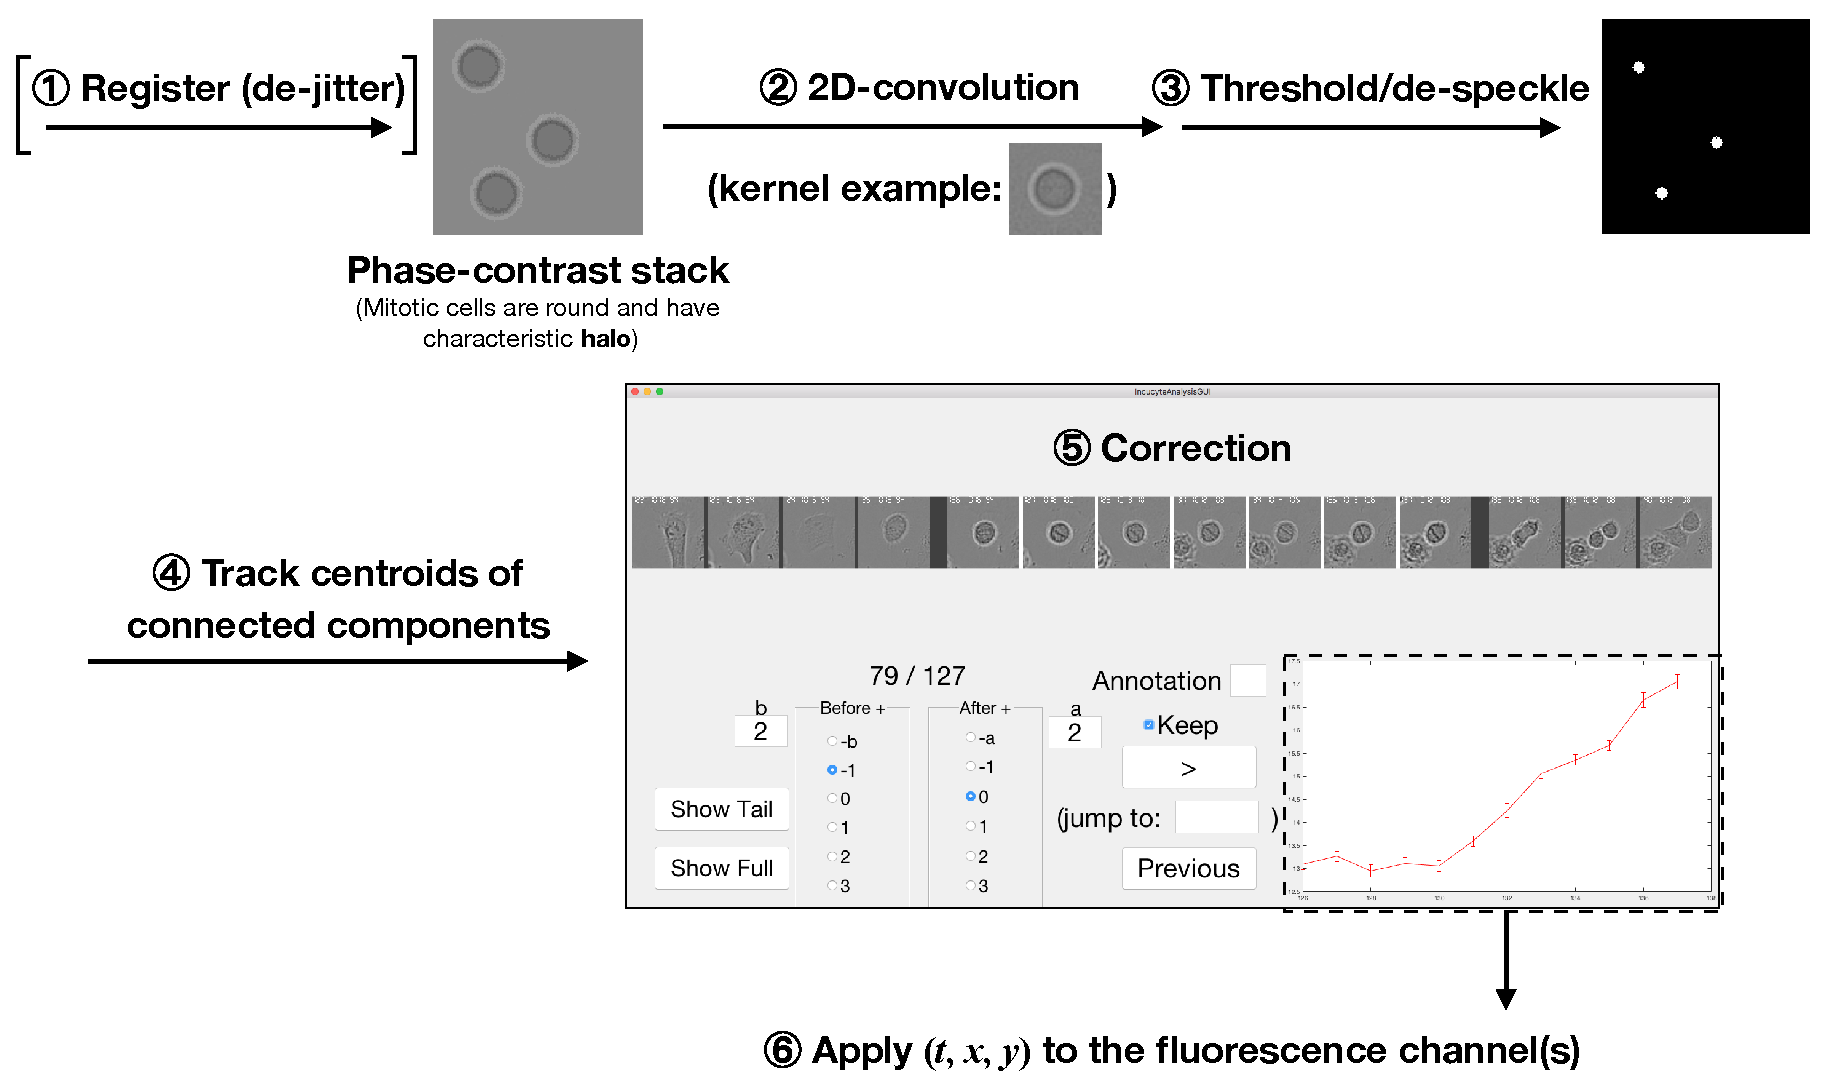
\includegraphics[width=0.95\textwidth]{chapters/figures/DataAnalysisPipeline.pdf}
    \caption{\textbf{A diagram illustrating the semi-automatic data analysis pipeline for mitotic duration assays.}}
    \label{DataAnalysisPipeline}
\end{figure}

\section{The eSAC activator reveals dose-response characteristics of the SAC}
The ability of the eSAC activator to hijack the endogenous SAC mechanism offered a novel tool to study the SAC quantitatively by correlating the cytosolic abundance of the eSAC activator with the mitotic duration from NEBD to anaphase onset (mitotic slippage) in a large population of cells. The first subject we explored was how the number of MELT motifs in the phosphodomain of \protein{Knl1} affects the signaling activity of the SAC (\myref{Summary_DoseResponse}). The idea has been explored in previous studies and came up naturally because there are 19 putative MELT motifs with various affinities to bind \protein{Bub1}-\protein{Bub3} in human \protein{Knl1} \cite{RecombinantKNL1, MELTActivity}.

\begin{figure}
    \centering
    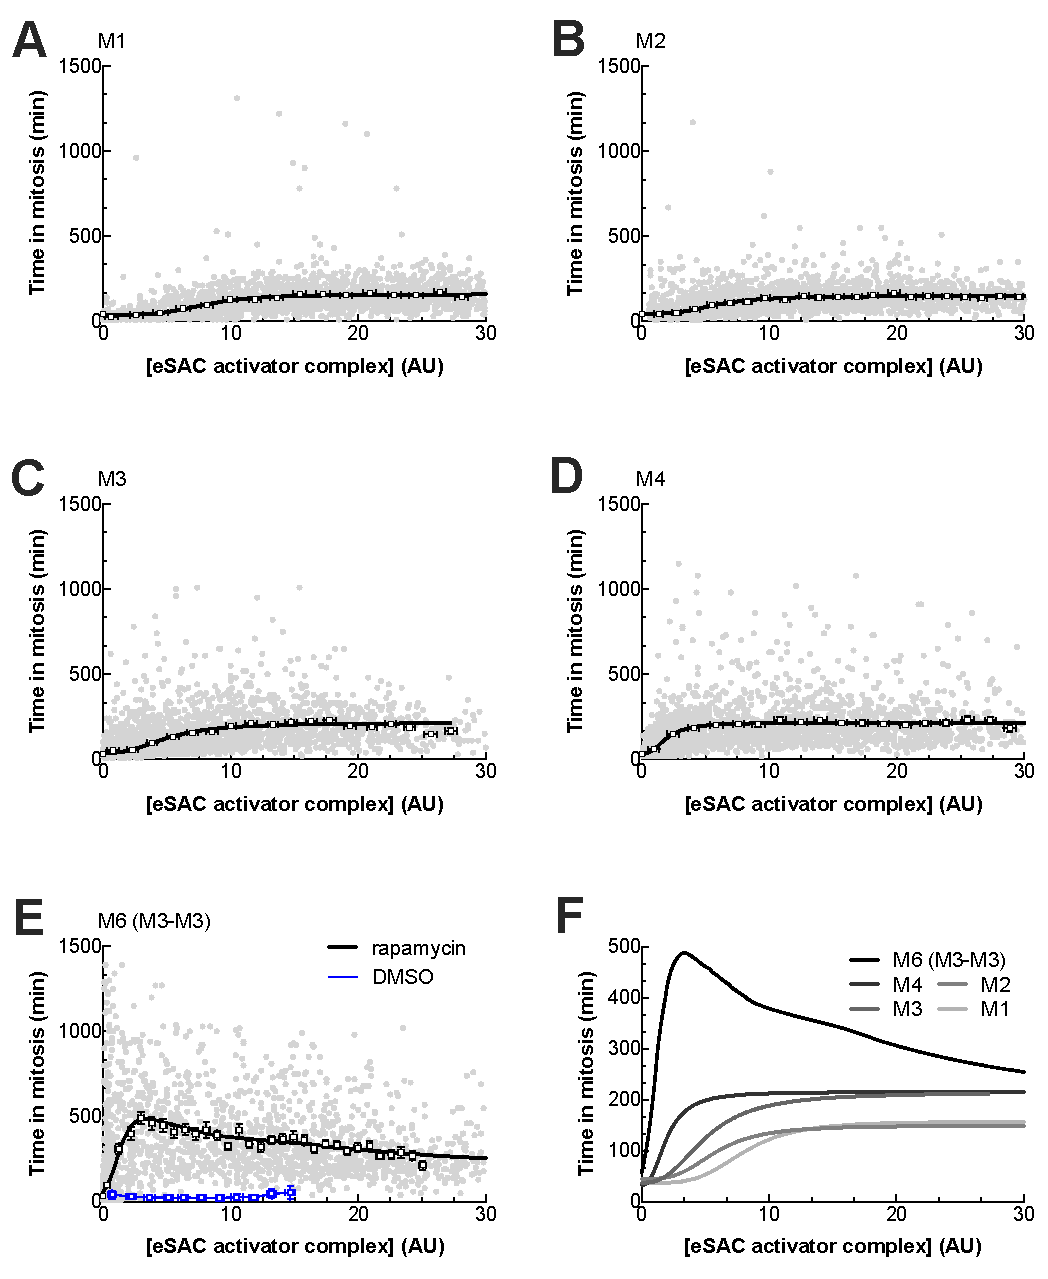
\includegraphics[width=0.7\textwidth]{chapters/figures/DoseResponse.pdf}
    \phantomsubfiglabel{M1_DoseResponse} % subfigure A
    \phantomsubfiglabel{M2_DoseResponse} % subfigure B
    \phantomsubfiglabel{M3_DoseResponse} % subfigure C
    \phantomsubfiglabel{M4_DoseResponse} % subfigure D
    \phantomsubfiglabel{M6_DoseResponse} % subfigure E
    \phantomsubfiglabel{Summary_DoseResponse} % subfigure F
    \caption{\textbf{A summary of the dose-response curves for the five eSAC activators with recombinant phosphodomains containing one to six MELT motifs.}}
    \noindent\justifying The dose (red fluorescence readout of the recombinant \protein{Mps1} kinase domain at the beginning of prometaphase in the cytosol of each cell) versus response (time in mitosis) relationship for different eSAC activators [(A) M1, (B) M2, (C) M3, (D) M4, and (E) M6 (M3-M3)]. Each gray dot represents a cell. Data from at least two independent experiments were compiled with more than \SI{2500}{} cells analyzed in each group. There may be some outliers beyond the range of the $x$- or $y$-axis (but they are included in the fitting). Bins of raw data (open squares, representing means $\pm$ SEMs) are overlaid. (F) shows a summary of the fitted dose-response curves for the five eSAC activators with recombinant phosphodomains containing one to six MELT motifs. Data from M1, M2, M3, and M4 are fitted to a Hill equation (see the main text) while LOESS (locally estimated scatterplot smoothing) was applied to show the trend of M6 (M3-M3). This figure is compiled and adapted from Figures 3C, 3E, 3F, 3G, 4B, and 4C of \cite{eSAC}. Dr. Ajit Joglekar, Adrienne Fontan, and Lauren Humphrey-Stark also contributed to setting up the experiments and/or performing data analysis.
    \label{DoseResponse}
\end{figure}

We started out by incorporating a single MELT motif (MELT\textsuperscript{12}, which is henceforth referred to as ``M1'', representing the minimal signaling unit of the core SAC signaling cascade) into the recombinant phosphodomain of the eSAC activator. We found that the duration of mitosis in the presence of \SI{500}{nM} rapamycin depended on the cytosolic abundance of the eSAC activator (\myref{M1_DoseResponse}). We used a Hill equation to fit these data, which displayed a sigmoidal trend:
\begin{equation*}
    \text{Time in mitosis} = m + \dfrac{M}{1+(\dfrac{K}{\text{[eSAC activator]}})^n},
\end{equation*}
wherein $n$ is the Hill coefficient and $K$ is the level of the eSAC activator at which the time in mitosis reaches the middle between the baseline level ($m$) and the plateau level ($m+M$).

Similar sigmoidal trends were also observed in dose responses of eSAC activators with recombinant phosphodomains containing two (MELT\textsuperscript{12}-MELT\textsuperscript{13}, henceforth referred to as ``M2''; \myref{M2_DoseResponse}), three (MELT\textsuperscript{12}-MELT\textsuperscript{14}, henceforth referred to as ``M3'' \cite{RecombinantKNL1}; \myref{M3_DoseResponse}), or four (MELT\textsuperscript{11}-MELT\textsuperscript{14}, henceforth referred to as ``M4''; \myref{M4_DoseResponse}) MELT motifs. The maximal mitotic duration for eSAC activators with recombinant phosphodomains containing one or two MELT motifs was the same, but it was higher for eSAC activators with recombinant phosphodomains containing three or four MELT motifs. Given that the eSAC activator recruits SAC proteins to arrest cells in metaphase, limited cytosolic abundance of one (or some) of the SAC proteins likely restricts the maximal mitotic duration (a metric of the signaling activity of the SAC), leading to a plateau at high abundance of the eSAC activator. This layer of restriction is coupled with diverse rates of MCC assembly, leading to various plateau levels for different recombinant phosphodomains (see \myref{ProzoneEffectModel,eSACDiscussions}). These results were consistent with a previous kinetochore-based study demonstrating that the \protein{Knl1} phosphodomain requires multiple MELT motifs to enable robust SAC signaling \cite{RecombinantKNL1}.

Surprisingly, the dose response of an eSAC activator with a recombinant phosphodomain containing six MELT motifs, which is made up of two tandem M3's and henceforth referred to as ``M6 (M3-M3)'' \cite{RecombinantKNL1}, featured a non-monotonic curve (\myref{M6_DoseResponse}). This eSAC activator induced a strong mitotic arrest at a low concentration. As the abundance of the eSAC activator complex increased, the signaling activity of the SAC gradually decreased.

\section{The distance between MELT motifs has a minor impact on the SAC activity}
There are two major differences between the M1, M3, and M6 (M3-M3) eSAC constructs in the previous section: (1) that the total number of MELT motifs in the signaling scaffold are different and (2) the lengths of these signaling scaffolds are different. Even though the phosphodomain of \protein{Knl1} is largely unstructured and flexible \cite{UnstructuredKNL1}, it remains to be seen whether the distance between MELT motifs affects the SAC activity. As a reference, the pair-wise distance between neighboring MELT motifs in the endogenous \protein{Knl1} are illustrated in \myref{PairwiseDistancesBetweenNeighboringMELTs}.

\begin{figure}
    \centering
    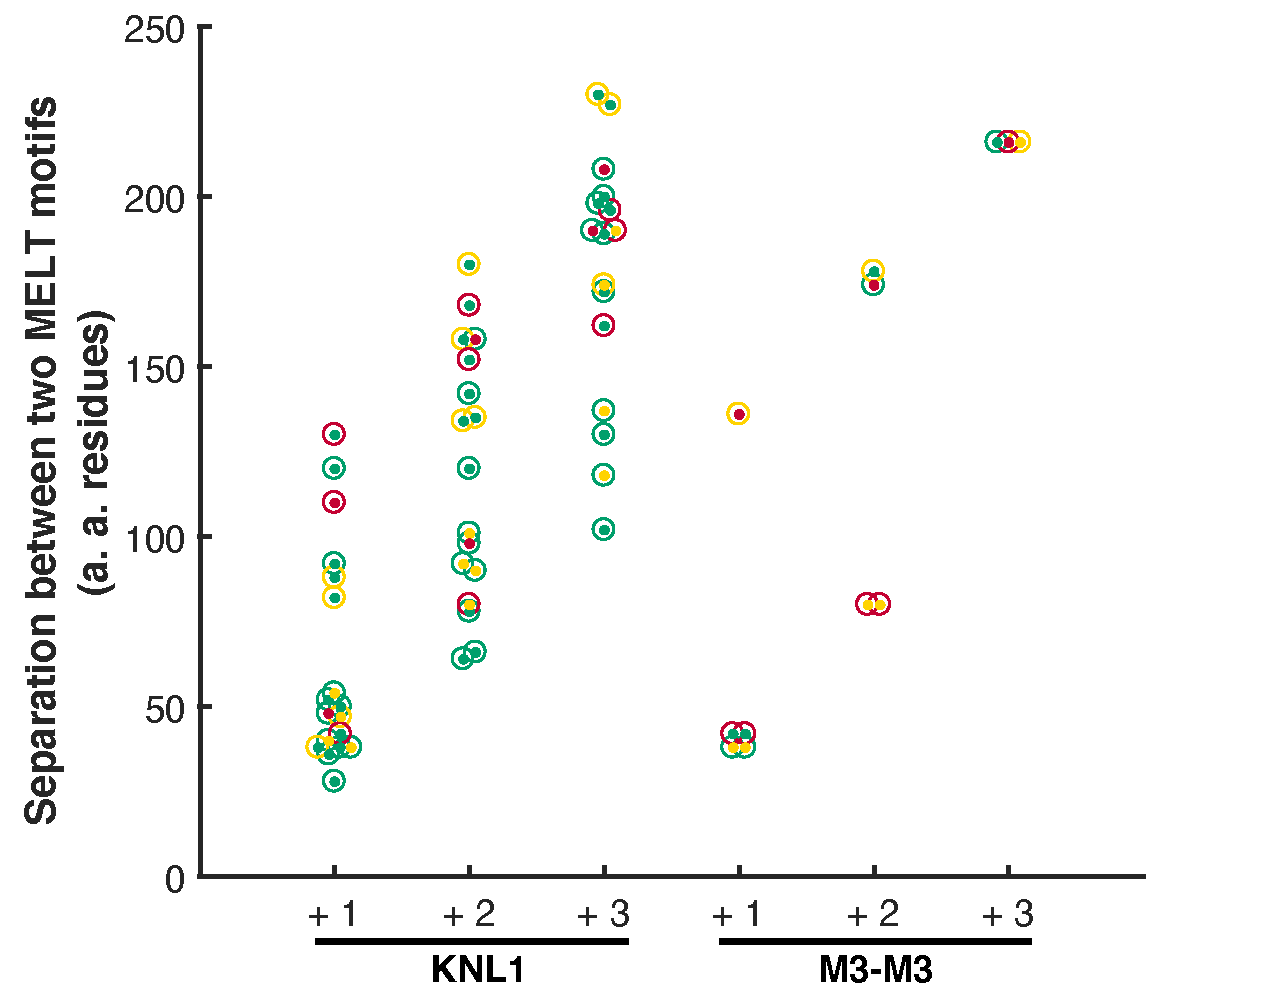
\includegraphics[width=0.6\textwidth]{chapters/figures/MELTSeparationColorCodedBeeSwarmPlot.pdf}
    \caption{\textbf{A beeswarm plot of pairwise distances between $(+1, +2, +3)$-neighboring MELT motifs in human \protein{Knl1} and the M6 (M3-M3) eSAC construct.}}
    \noindent\justifying Each ``circle \& center'' symbol represents a pair of neighboring MELT motifs. There are a total number of 19 putative MELT motifs in the endogenous \protein{Knl1} and 6 MELT motifs in the signaling scaffold of the M6 (M3-M3) eSAC construct. Therefore, we have a total number of $(18, 17, 16)$ pairs and $(5, 4, 3)$ pairs of $(+1, +2, +3)$-neighboring MELT motifs in the endogenous \protein{Knl1} and the M6 (M3-M3) eSAC construct, respectively. The coloring scheme follows the one in the original research \cite{MELTActivity} that studies the recruitment of \protein{Bub1} and is a rough estimation of the signaling activity of the corresponding MELT motifs (green: ``high'', yellow: ``intermediate'', red: ``low''). Distances in this chapter are measured between the Thr/Ser's of the consensus ``MELT'' sequences.
    \label{PairwiseDistancesBetweenNeighboringMELTs}
\end{figure}

To study the effect of the distance between MELT motifs in the signaling scaffold on the SAC activity, we designed a series of eSAC assays using artificially designed signaling scaffolds [MELT\textsuperscript{12}-$1\times$linker-MELT\textsuperscript{12}, MELT\textsuperscript{12}-$2\times$linker-MELT\textsuperscript{12}, and MELT\textsuperscript{12}-$3\times$linker-MELT\textsuperscript{12}]. The total number of MELT motifs are fixed (two) and the sequence of MELT motifs adopts that of MELT\textsuperscript{12}. Various copies of the endogenous linker between MELT\textsuperscript{11} and MELT\textsuperscript{12} are inserted between the two MELT\textsuperscript{12}'s. The resulting distance between the two MELT\textsuperscript{12}'s varies from 135 to 311 amino acids (\myref{DistanceEffect}), compared to a distance of 296 amino acids between the first motif and the last MELT motif in the M6 (M3-M3) construct in the previous section. From these assays, we observed that MELT\textsuperscript{12}-$3\times$linker-MELT\textsuperscript{12} has a slightly less SAC activity compared to the other two, but the difference is small and negative (about \SI{-15}{min} to \SI{-10}{min}) compared to the differences in the SAC activities between M1 and M6 (M3-M3) [as well as between M3 and M6 (M3-M3)]. Therefore, we inferred that the difference in the number of MELT motifs in the eSAC constructs is the major factor that determines its SAC activity.

\begin{figure}
    \centering
    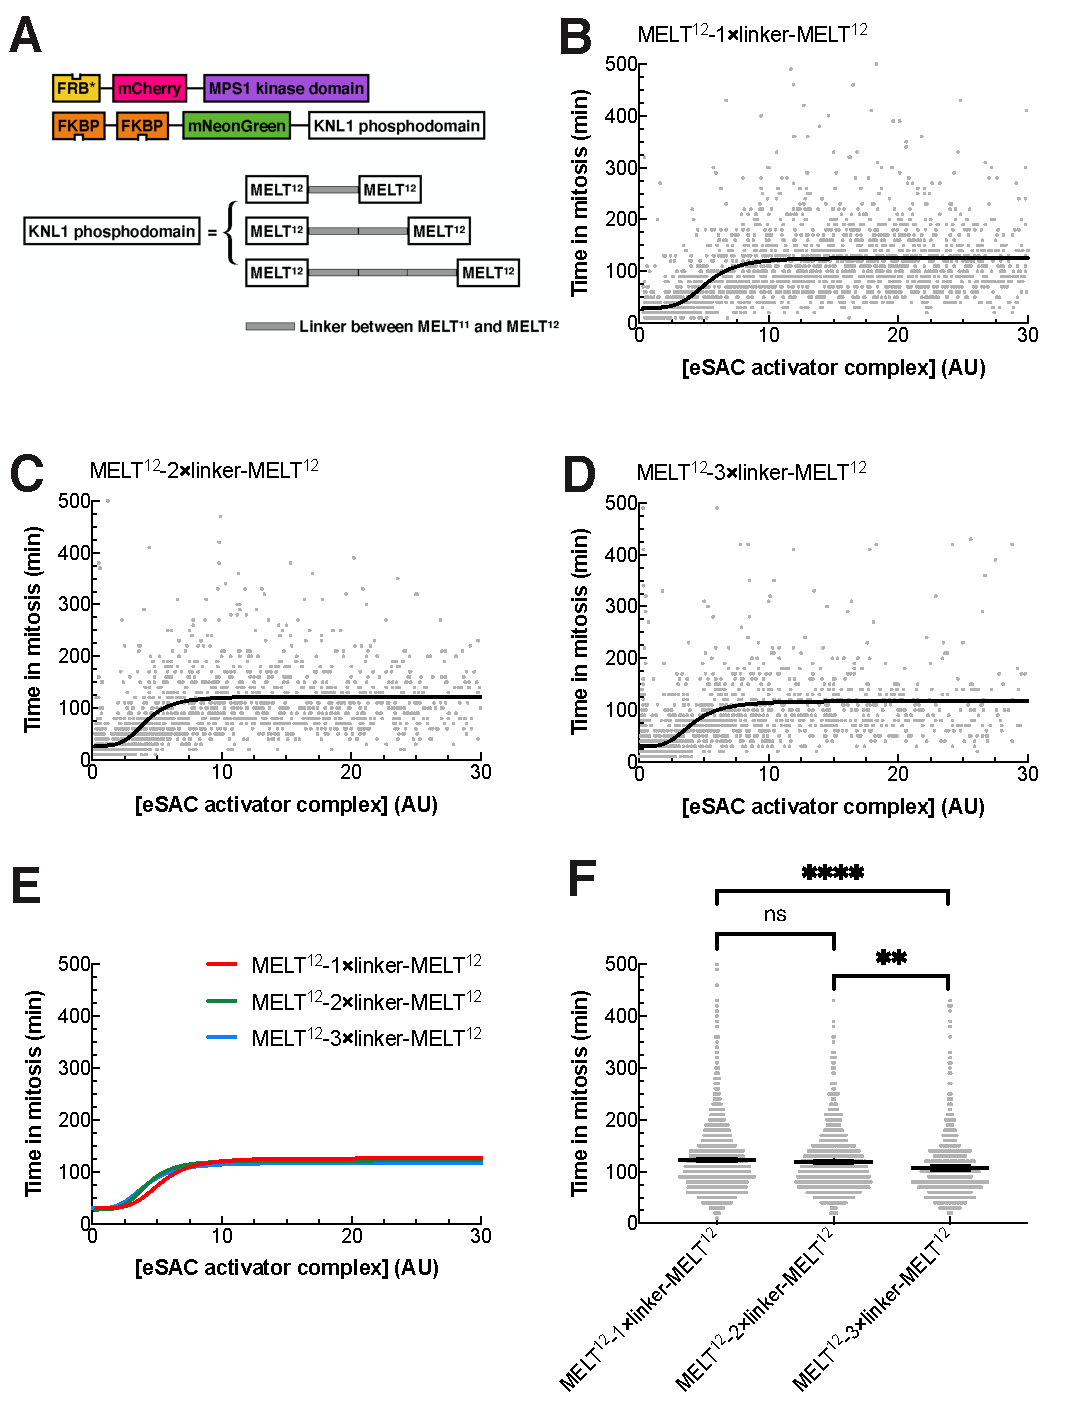
\includegraphics[width=0.7\textwidth]{chapters/figures/DistanceEffect.pdf}
    \caption{\textbf{The distance between MELT motifs has a minor impact on the SAC activity.}}
    \noindent\justifying (A) The distance between the two MELT\textsuperscript{12} motifs in the three constructs are 135, 223, and 311 amino acids, respectively [compared to a distance of 296 amino acids between the first motif and the last MELT motif in the M6 (M3-M3) construct in the previous section]. (B-E) A summary (E) of eSAC activities of MELT\textsuperscript{12}-$1\times$linker-MELT\textsuperscript{12} (B), MELT\textsuperscript{12}-$2\times$linker-MELT\textsuperscript{12} (C), and MELT\textsuperscript{12}-$3\times$linker-MELT\textsuperscript{12} (D) as the signaling scaffold. Each gray dot represents a cell. There may be some outliers beyond the range of the $x$- or $y$-axis (but they are included in the fitting).  (F) Comparison of the plateau levels of SAC response curves of the three eSAC constructs. Only cells with [eSAC activator] $> 10$ AUs are included. Data of more than 500 cells from two independent experiments were pooled for each group. The average mitotic durations are $(122.3 \pm 3.4)$, $(119.1 \pm 4.4)$, and $(108.1 \pm 5.7)$ minutes. The mean value $\pm$ the 95\% confidence interval of each group is overlaid. Unpaired $t$-tests with Welch's correction were performed in Prism 9 (GraphPad Software).
    \label{DistanceEffect}
\end{figure}

\section{The dose-response data suggest cooperativity between multiple MELTs on a \protein{Knl1} phosphodomain that boosts the SAC signaling activity}
\label{ProzoneEffectModel}
We hypothesized that the increase in the maximum signaling activity of the recombinant \protein{Knl1} phosphodomain with multiple MELT motifs indicates synergistic signaling. This cooperativity model enables eSAC activator to assemble MCC at a higher rate than what independent signaling of the MELT motifs may sum up to. In fact, if each individual MELT motif on a recombinant \protein{Knl1} phosphodomain generates the MCC independently, the dose response of an eSAC activator with a recombinant phosphodomain containing a larger number of MELT motifs will simply approach the same plateau level of SAC activity at a lower concentration of the eSAC activator. This reasoning is especially evident when we compare the dose response of M3 (\myref{M3_DoseResponse}) eSAC versus the dose response of M6 (M3-M3, \myref{M6_DoseResponse}) eSAC.

As the concentration of the eSAC activator increases, they compete with each other to recruit SAC proteins from their limited pools in the cytosol. Individual eSAC activators, even with multiple phosphorylated MELT motifs, may not be able to bind multiple SAC proteins concurrently. Thus, the synergistic SAC signaling dwindles. This model explains the dramatic decline in the dose response of the M6 (M3-M3) eSAC activator at high concentrations (\myref{M6_DoseResponse}), which is reminiscent of the hook effect \cite{HookEffect}.

\section{Discussions}
\label{eSACDiscussions}
As an analogous system, the cytosolic eSAC activator provides a convenient approach to study the design of the core SAC signaling cascade quantitatively in mammalian cells. A previous study demonstrated that M6 (M3-M3) had similar SAC signaling activity to the endogenous human \protein{Knl1} phosphodomain (containing a total number of 19 putative MELT motifs) in Flp-In HeLa cells expressing LAP-\protein{Knl1} variants \cite{RecombinantKNL1}. Critical insights provided by dose-response data for eSAC activators with various recombinant phosphodomains hint on how the core signaling cascade of the SAC may adapt the signaling activity of each kinetochore based on the total number of signaling kinetochores in the cell.

Although the maximal response from the SAC signaling cascade saturates, its magnitude is not the same for all eSAC systems. This magnitude may be partially influenced by the rate of MCC assembly of various MELT motifs (the actual sequences of MELT\textsuperscript{11}, MELT\textsuperscript{12}, MELT\textsuperscript{13}, and MELT\textsuperscript{14} deviate from each other). A study published more recently from our lab on the sequence specificity of MELT motifs in Spc105 (the analog of human \protein{Knl1} in \Latin{Saccharomyces cerevisiae}) showed that replacing MELT motifs in Spc105 with those that bind to Bub1-Bub3 with a higher affinity reduces the possibility of chromosome missegregation but also slows down the progression of the cell cycle in the budding yeast \cite{YeastMELTSpecificity}. The evolution of MELT motif sequences may reflect a process of adjusting the balance between the accuracy of chromosome segregation and the propagation rate \cite{MELTEvolution}.

Using our dose-response data, we proposed a model for the biochemical design of the SAC signaling cascade. When there are a large number of signaling kinetochores in the cell (for example, right after NEBD), they compete with each other in recruiting SAC proteins from their limited pools in the cytosol. This competition masks cooperativity and the SAC activity per signaling kinetochore is weak. However, because the number of signaling kinetochores is large, the SAC signaling activity is high. When there are a few or even a single signaling kinetochores in the cell (for example, at a later stage of the prometaphase), each signaling kinetochore or even each \protein{Knl1} at signaling kinetochores can now recruit a large number of SAC proteins at the same time and cooperativity enables each remaining signaling kinetochores to assemble MCC at a high rate.

Unstable association between the recombinant \protein{Knl1} phosphodomain and the recombinant \protein{Mps1} kinase domain may introduce a source of noise. Therefore, we built upon the rapamycin-induced dimerization system to engineer our eSAC activator. However, endogenous \protein{Mps1} competes with microtubules to bind to the \protein{Ndc80} complex, thereby gaining spatial proximity to \protein{Knl1} at kinetochores \cite{MPS1Localization_Ji, MPS1Localization_Hiruma}. It is possible that the difference in the dynamics of \protein{Mps1} could potentially lead to observation of artifacts that do not apply to the endogenous SAC signaling cascade. Therefore, the model proposed here should be rigorously examined on kinetochore-based SAC signaling. This is the motivation of our study described in \myref{chpt:3}.

\section{Materials and Methods}
\subsection{Purification of the recombinant \protein{Mps1} kinase domain}
The recombinant bacmid encoding 6×His-MBP-TEV-FRB*-mCherry-\protein{Mps1}\textsuperscript{kinase domain} (\SI{124.8}{kDa}) was generated %from pCCB15
via Bac-to-Bac\textsuperscript{\textregistered} (Thermo Fisher Scientific). Baculovirus-transfected Sf9 cells (from \SI{1}{L} of culture) were pelleted down and stored at \SI{-80}{\celsius} until protein purification. Cells were resuspended in buffer IA [\SI{50}{mM} Tris-HCl (pH 7.5), \SI{300}{mM} NaCl, 0.2\% Triton X-100, \SI{20}{mM} imidazole, 0.1\% \textbeta-mercaptoethanol, and supplemented with PMSF and cOmplete\texttrademark{} EDTA-free Protease Inhibitor Cocktail (Roche) before usage] to a total volume of \SI{60}{mL}. Cells were lysed by a Dounce homogenizer (20 strokes using the loose pestle followed by 1 stroke using the tight pestle) supplied with Benzonase\textsuperscript{\textregistered} Nuclease (Sigma-Aldrich). Cell lysates were then centrifuged at \SI{18000}{rpm}, \SI{4}{\celsius} for \SI{45}{min} in a F21S-8x50y rotor. The supernatant was transferred and the pellet was discarded. \SI{5}{mL} of Ni-NTA agarose (equilibrated with buffer IA; Thermo Fisher Scientific) was added into the supernatant and the mixture was rotated at \SI{4}{\celsius} for \SI{3.5}{h}. The slurry was then washed with \SI{5}{mL} of buffer IA for 4 times. Bound proteins were eluted with buffer IB [\SI{50}{mM} Tris-HCl (pH 7.5), \SI{300}{mM} NaCl, 0.2\% Triton X-100, \SI{200}{mM} imidazole, 0.1\% \textbeta-mercaptoethanol].

\SI{2}{mL} of amylose resin was added (equilibrated with buffer IB; New England Biolabs) into eluted proteins from the Ni-NTA agarose column and the mixture was rotated at \SI{4}{\celsius} for \SI{2.5}{h}. The protein-bound amylose resin was then washed with \SI{5}{mL} of buffer IC [\SI{50}{mM} Tris-HCl (pH 7.5), \SI{300}{mM} NaCl, 0.2\% Triton X-100] for 4 times. \SI{2.5}{mL} of buffer IC followed by \SI{40}{\micro L} of \SI{1}{M} \textsc{d}-(+)-maltose stock solution was then added into the slurry. The mixture was rotated at \SI{4}{\celsius} for \SI{30}{min} and then eluted proteins were collected. The elution was loaded onto a Superdex 200 pg column (Cytiva) for size-exclusion chromatography. Fractions corresponding to the monomeric full-length 6×His-MBP-TEV-FRB*-mCherry-\protein{Mps1}\textsuperscript{kinase domain} (determined by molecular weight estimation and SDS-PAGE analysis) were subject to a subsequent Bradford protein assay (Bio-Rad Laboratories) and later used in the in vitro kinase assay.

\subsection{Purification of the recombinant \protein{Knl1} phosphodomain}
%pCCB9-
Transformed Rosetta\texttrademark{} 2(DE3) cells were induced to express 6×His-3×FLAG-TEV-MELT\textsuperscript{12-14}-mNeonGreen-2×FKBP (\SI{73.1}{kDa}) by \SI{1}{mM} IPTG at \SI{25}{\celsius} for \SI{20}{h}. Cells from \SI{2}{L} of Luria-Bertani liquid media were harvested, resuspended in deionized water into a total volume of \SI{40}{mL}, and then stored at \SI{-80}{\celsius} until protein purification.

The cell slurry was thawed on ice and an equal volume of $2\times$ buffer A [the $1\times$ buffer A has the following composition: \SI{50}{mM} Tris-HCl (pH 7.4), \SI{500}{mM} NaCl, \SI{0.1}{mM} EDTA, \SI{0.1}{mM} EGTA, and \SI{20}{mM} imidazole] supplemented with PMSF, \SI{0.1}{mg/mL} chicken egg white lysozyme (Sigma-Aldrich), \SI{2}{mM} DTT, and cOmplete\texttrademark{} EDTA-free Protease Inhibitor Cocktail was added into the slurry. Cells were lysed by sonication for a total amount of on time of \SI{150}{s} at 62\% amplitude (Model 500 sonic dismembrator, Thermo Fisher Scientific) in a water-ice bath at \SI{0}{\celsius}. Triton X-100 was added to a final concentration of 0.5\%. Lysates were rotated for \SI{15}{min} and then centrifuged at \SI{18000}{rpm}, \SI{4}{\celsius} for \SI{45}{min} in a F21S-8x50y rotor. The supernatant was filtered through 0.45-\textmu{}m syringe filter units (MilliporeSigma) and the pellet was discarded. \SI{1.5}{mL} of Ni-NTA agarose (equilibrated with buffer A supplemented with 0.1\% Triton X-100) was added into the filtered supernatant and the mixture was rotated at \SI{4}{\celsius} for \SI{3}{h}. The slurry was then washed with \SI{10}{mL} of buffer A supplemented with 0.1\% Triton X-100 for 4 times. Bound proteins were eluted with \SI{6}{mL} of buffer B [\SI{50}{mM} Tris-HCl (pH 7.4), \SI{500}{mM} NaCl, \SI{0.1}{mM} EDTA, \SI{0.1}{mM} EGTA, 0.1\% Triton X-100, and \SI{200}{mM} imidazole] for \SI{1}{h} at \SI{4}{\celsius}. The elution was filtered through a 0.45-\textmu{}m syringe filter unit and dialyzed in a Slide-A-Lyzer\texttrademark{} dialysis cassette (10K MWCO; Thermo Fisher Scientific) overnight against an imidazole-free buffer [\SI{50}{mM} Tris-HCl (pH 7.45 at \SI{4}{\celsius}) and \SI{300}{mM} NaCl] and then loaded onto a Superdex 200 pg column for size-exclusion chromatography. Fractions corresponding to the 6×His-3×FLAG-TEV-MELT\textsuperscript{12-14}-mNeonGreen-2×FKBP (determined by molecular weight estimation and SDS-PAGE analysis) were later used in the in vitro kinase assay.

\subsection{In vitro kinase assay}
The substrate 6×His-3×FLAG-TEV-MELT\textsuperscript{12-14}-mNeonGreen-2×FKBP was incubated with 6×His-MBP-TEV-FRB*-mCherry-\protein{Mps1}\textsuperscript{kinase domain} at \SI{30}{\celsius} for \SI{5}{min} -- \SI{2}{h} in the kinase buffer [\SI{10}{mM} Tris-HCl (pH 7.5), \SI{100}{mM} NaCl, \SI{10}{mM} \ch{MgCl2}, and \SI{1}{mM} DTT] supplemented with \SI{500}{nM} rapamycin and \SI{0.25}{mM} ATP. The reactions were stopped with the Laemmli Sample Buffer (supplemented with \textbeta-mercaptoethanol, Bio-Rad Laboratories). Phosphorylation of the substrate was detected by our custom-made anti-\Peptide{MEIpTRSHTTALEC} phospho-specific rabbit polyclonal antibody (GenScript). Equal inputs of the substrate and the recombinant kinase across different groups were validated by silver staining (Bio-Rad Laboratories).

\subsection{Cell culture and Cre-\bacterialgene{lox} recombination-mediated cassette exchange}
All HeLa-A12 cells were cultured in Dulbecco's Modified Eagle's Medium (DMEM, with high glucose and phenol red, without glutamine, sodium pyruvate, or HEPES; Gibco) supplemented with 22 mM of HEPES (Corning), 9\% (by volume) of fetal bovine serum (Corning), and $1\times$ GlutaMAX (Gibco). This medium is referred to as ``complete DMEM'' in the following context.

For Cre-\bacterialgene{lox} RMCE, Lipofectamine 3000 (Invitrogen) is used to co-transfect \SI{1.5}{\micro g} of a circular plasmid carrying the transgene cassette and \SI{50}{ng} of the circular pCAGGS-nlCre plasmid. \SI{0.5}{\micro g/mL} of puromycin was added \SI{1.5}{d} later for \SI{3}{d} to select for stably-transfected HeLa-A12 cells. Puromycin-resistant colonies were then pooled together and subject to further validation by genotyping and/or immunoblotting.

\subsection{live-cell imaging on the IncuCyte\textsuperscript{\textregistered} ZOOM system}
Long-term fluorescence imaging of eSAC cell lines was conducted using the IncuCyte\textsuperscript{\textregistered} ZOOM Live Cell Analysis System (Sartorius) equipped with a $20\times$ objective. Cells were seeded in 12-well BioLite cell culture-treated plates (Thermo Fisher Scientific) 2 days before imaging in complete DMEM supplemented \SI{2}{\micro g/mL} doxycycline. 30 -- 60 minutes prior to imaging, cells were washed once and FluoroBrite\texttrademark{} DMEM [supplemented with 9\% (by volume) of fetal bovine serum (Corning) and \SI{2}{\micro g/mL} doxycycline] with or without \SI{500}{nM} rapamycin were added. Phase-contrast and fluorescence images were acquired every \SI{10}{min} at fixed positions.% Images of the red and green fluorescence channels were acquired using a fixed exposure time of \SI{900}{ms} and \SI{300}{ms}, respectively.